%==============================================================================
\chapter{Detector}
\label{sec:det}
%==============================================================================

In this chapter, a detailed description of the proposed PINGU neutrino
telescope and its predecessor IceCube will be given. We will start with
introducing the concept of ice or water based neutrino telescopes based on the
detection of Cherenkov radiation with IceCube/DeepCore as example, followed by
a characterisation of its upcoming PINGU upgrade.
Thereafter we will discuss how physics events will be selected and
reconstructed in an analysis targeting the determination of the neutrino mass
hierarchy, and finally how conceptually new hardware might improve the results.

%==============================================================================
\section{IceCube/DeepCore}
\label{sec:ICDC}
%==============================================================================

\subsection{Location}
\label{sec:IClocation}

As already mentioned (Sec.~\ref{sec:NuDetection}), the natural choice for
observing the low natural fluxes of high energy neutrinos are water-based
Cherenkov detectors. Although the basic requirement---a sufficiently large
amount of water or ice---seems not very difficult to meet, there are additional
constraints that have to be addressed as well:

\begin{description}
 \item[Size:] Depending on the energy range one is interested in, the size of
  the detector has to be adjusted accordingly. Since the atmospheric flux
  decreases rapidly with increasing energy, one needs larger detectors to study
  higher fluxes. Roughly from the GeV scale upwards, the required dimensions are
  so big (several hundred metres) that artificial structures like the
  underground caverns of Kamiokande and Super-Kamiokande \cite{SuperKosc} are
  not feasible any more and one has to look for suitable natural locations.
 \item[Transparency:] Since the detection of neutrinos is based on recording
  Cherenkov radiation, i.\,e.\ photons in the optical and near UV regime,
  obviously the chosen medium has to be transparent for these photons. Here ice
  has an advantage over fluid water as it has very low absorption down to
  wavelengths of 300\,nm and below \cite{IceProps}, while the fluid starts to
  absorb significantly below 400\,nm \cite{WaterAbs}.
 \item[Purity:] Usually the experiments try to reconstruct the neutrino events
  as accurately as possible. Therefore it is desirable to record a large number
  of unscattered photons and hence a very clear environment\footnote{There might
  be, however, situations where scattering is desired, e.\,g.\ when only the
  neutrino energy is of interest, then strong scattering keeps the photons
  inside the detector for a longer time and hence increases the total number
  of detected photons, thereby improving the energy resolution}.
 \item[Shielding:] In high energy neutrino experiments, muons from atmospheric
  showers created by cosmic radiation (cf.\ Sec.~\ref{sec:AtmNus}) are a
  background process whose rate is several orders of magnitude higher than the
  neutrino signal. In order to suppress those muons, detectors have to be
  placed deep underground so that there is a shielding with several hundred
  meters thickness, comparable to the range of $\mathcal{O}
  (100\,\mathrm{GeV})$ muons.
\end{description}

\begin{figure}[htp]
 \centering
 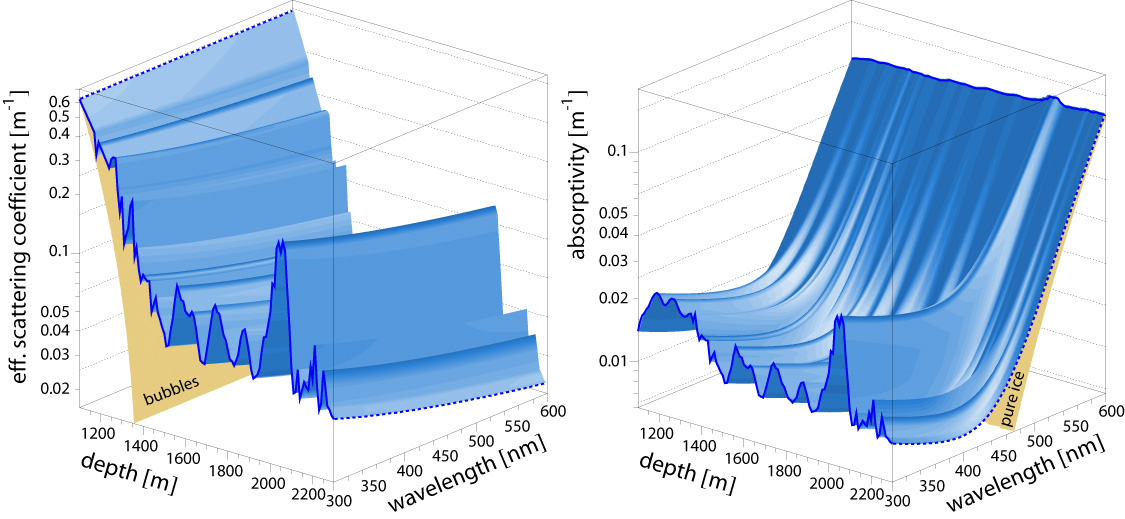
\includegraphics[width=\textwidth]{Icepaper_figure22_scatt-abs-length}
 \caption{Effective scattering and absorption of light in the polar ice. Plot 
  taken from \cite{IceProps}.}
 \label{fig:ice_scatt_abs}
\end{figure}

Choosing an environment optimising all these factors, the IceCube neutrino 
observatory has been constructed in the deep glacial ice at the geographical 
South Pole in Antarctica. The Antarctic glacier with its thickness of $\approx 
2500$\,m is a pristine environment of substantial size. In contrast to natural 
resources like lakes or the deep sea, it inherently provides a solid holding 
structure for the instrumentation, is free of lifeforms that might disturb or 
even destroy the detector, and has a much lower content of radioactive $^{40}$K 
than sea water. Especially at depths more than $\approx 2000$\,m below the 
surface, age and high pressure have facilitated the hydratisation of enclosed 
air bubbles, leaving an extremely clear ice with scattering and absorption 
lengths of several tens of metres even in the UV range, see 
Fig.~\ref{fig:ice_scatt_abs}. Instrumenting only the deepest ice below 1500\,m 
guarantees a sufficient shielding of atmospheric muons. 

The nearby Amundsen-Scott South Pole Station operated by the United States 
Antarctic Program provides the infrastructure needed for such a large scale 
experiment. This incorporates the supply of electrical power for the detector 
itself and the computing farm processing the raw data, satellite communications 
for transmitting science data, general technical support as well as 
accommodations for the visiting scientists.

\subsection{Detector Geometry}
\label{sec:ICgeometry}

A total of 86 strings, each instrumented with 60 Digital Optical Modules (DOMs, 
see Sec.~\ref{sec:ICDOM}), have been installed during IceCube's deployment phase 
from 2005 until December 18, 2010. A hot water drill was used to melt holes of 
60\,cm diameter into the ice, reaching down to 2450\,m, shortly above the 
underlying bedrock. Then the strings were lowered into the holes still filled 
with water which then refroze and firmly encloses the strings.

Eighty of those strings form the hexagonal main array with an inter-string 
distance of 125\,m, while the remaining six are placed at additional positions 
near the centre of the array, forming a dense sub-array with a string spacing 
of only 72\,m, lowering the threshold energy for neutrino detection from 
$\approx 100$\,GeV to $\approx 20$\,GeV. A top view of the string layout is 
shown in Fig.~\ref{fig:string_layout}.

\begin{figure}[htp]
 \centering
 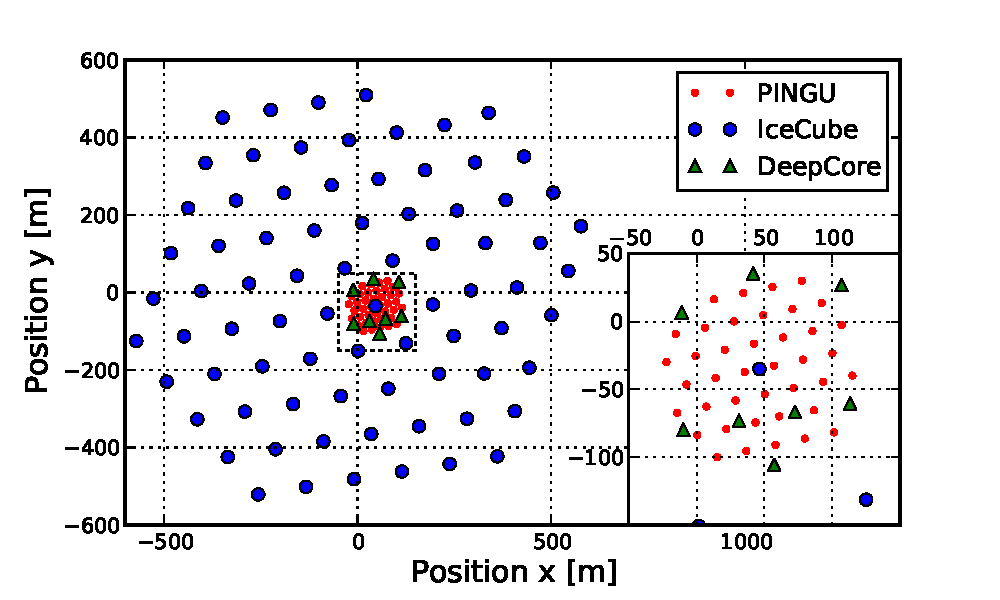
\includegraphics[width=\textwidth]{ic_dc_pingu_strings}
%  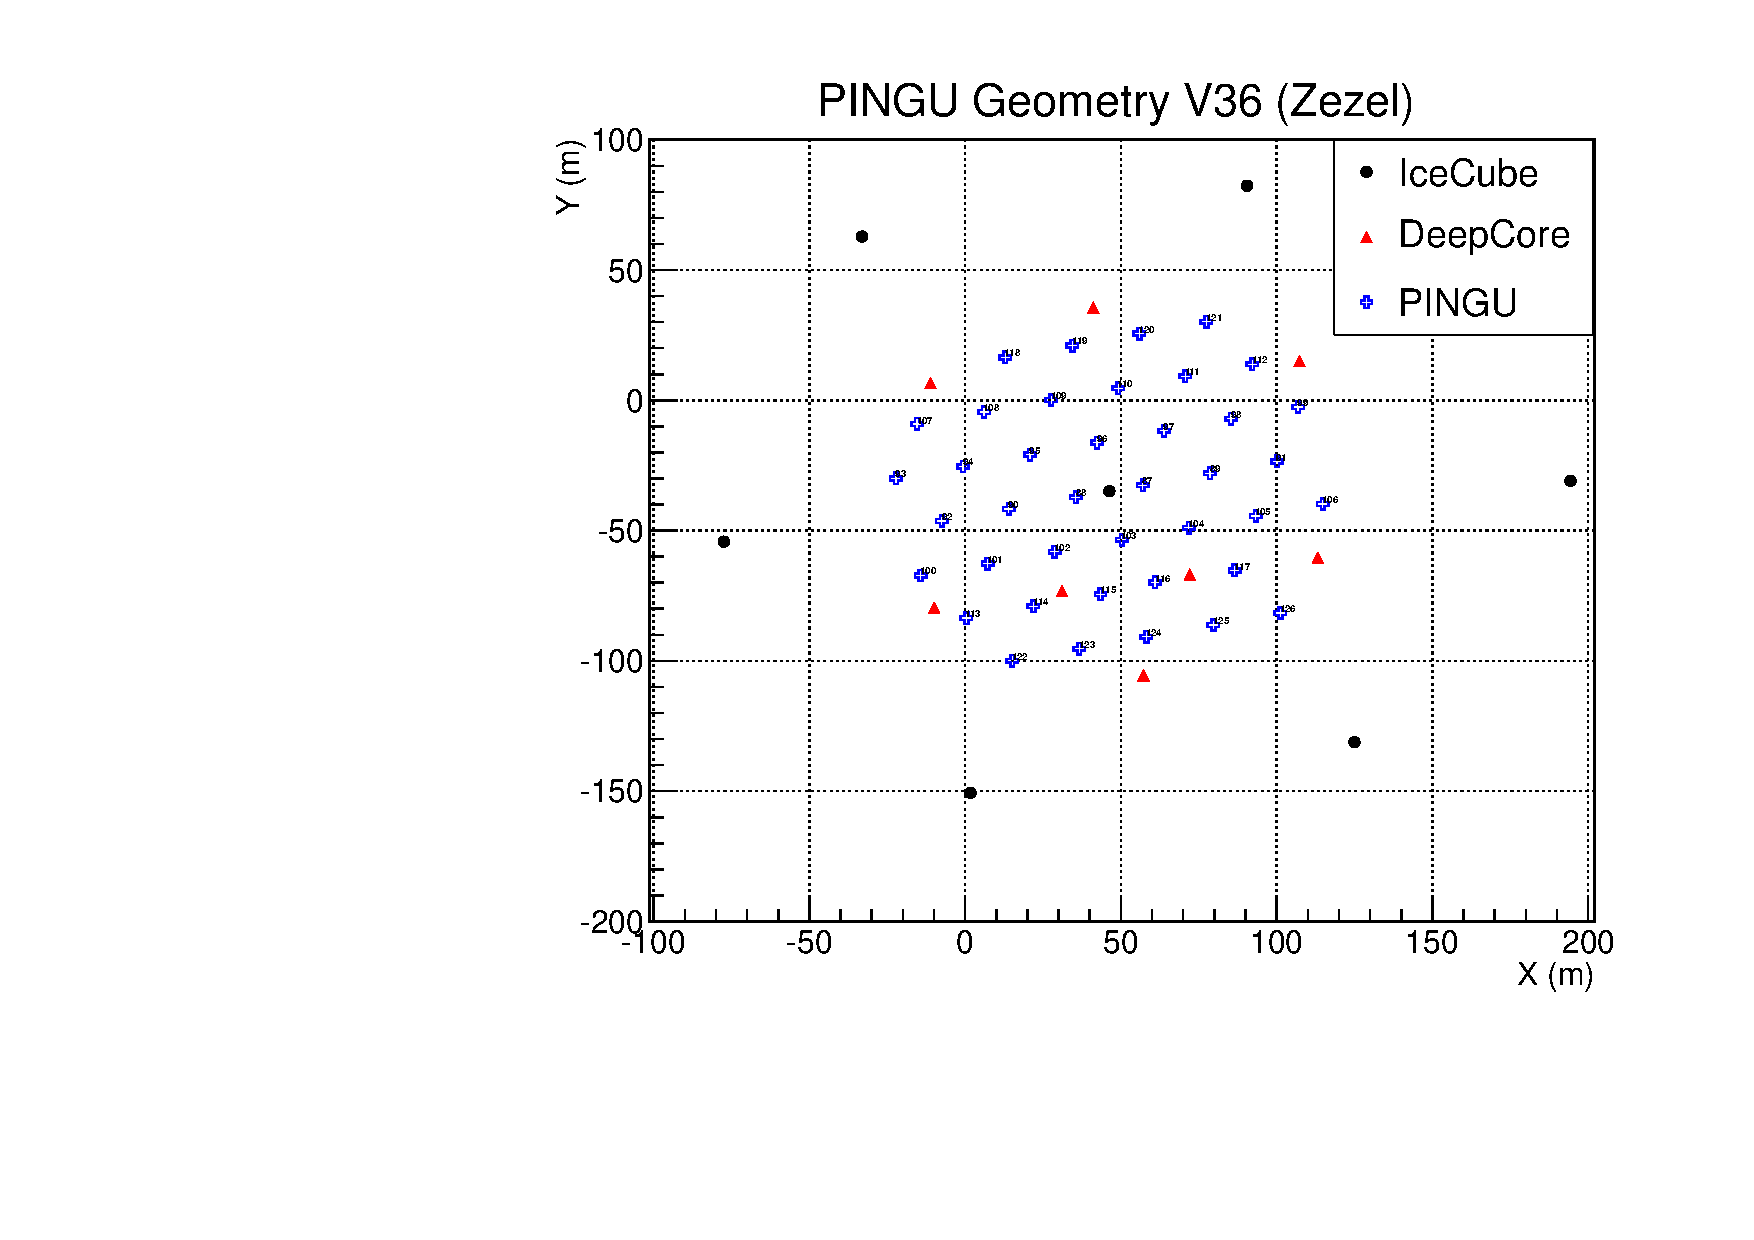
\includegraphics[width=0.7\textwidth]{pingu_V36_Zezel_40_s22_d3}
 \caption{Top view of the IceCube string layout, including the DeepCore and 
planned PINGU (geometry V36) sub-arrays.}
 \label{fig:string_layout}
\end{figure}

To the lowest 1000\,m of the main array strings, sixty DOMs each are attached, 
evenly spaced with a distance of 17\,m. In DeepCore, the vertical DOM spacing 
is only 7\,m below the dust layer found between 1950\,m and 2100\,m 
depth\footnote{The dust layer can be recognised easily in 
Fig.~\ref{fig:ice_scatt_abs} as the region of increased scattering and 
absorption.}, with a veto cap of ten DOMs with 10\,m spacing per DeepCore 
string above it \cite{I3Design,DCDesign}.


\subsection{Digital Optical Modules}
\label{sec:ICDOM}

\begin{figure}[htp]
 \centering
 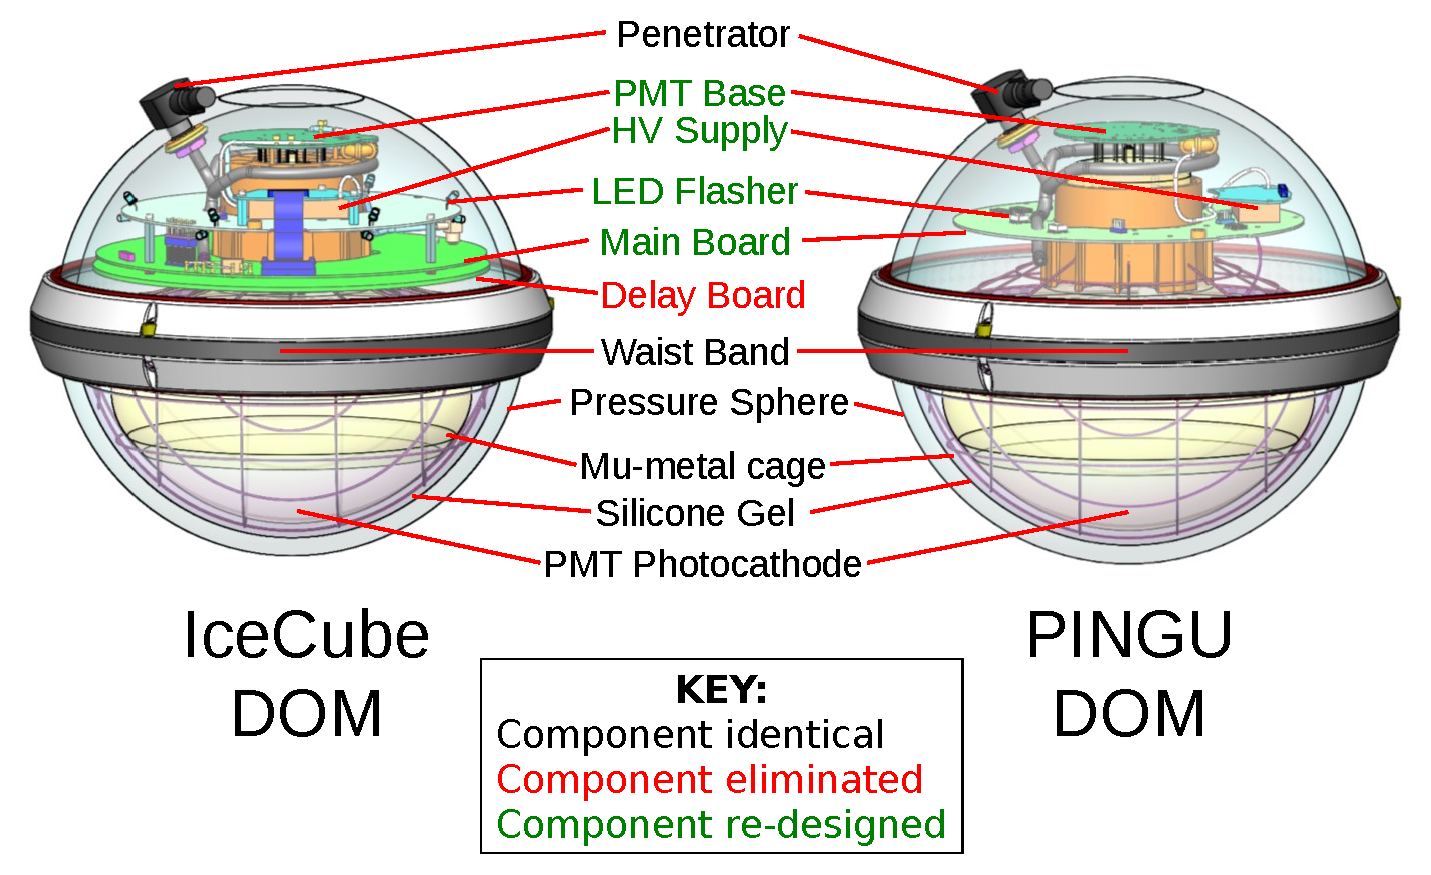
\includegraphics[width=0.7\textwidth]{I3DOM_PDOM_cropped}
 \caption{Comparing an IceCube/DeepCore DOM to the PDOM used in PINGU. Graphics 
taken from \cite{PDOM_Aachen}.}
 \label{fig:DOM}
\end{figure}

The 5160 Digital Optical Modules are the basic detection units of IceCube. They 
are attached to the string and connected to the main string cable during 
deployment and work autonomously except for the low voltage power supply. This 
modular design has the convenience that if one DOM fails to work and cannot be 
fixed as it is frozen in the deep ice, the others are not affected.

As shown in Figure \ref{fig:DOM}, the DOM is housed by a borosilicate glass 
sphere of 13\verb+"+ diameter and 0.5\verb+"+ thickness to withstand the 
pressure arising from the refreezing water in the drill holes. This glass sphere 
also contributes to the noise rate of about 540\,Hz per DOM as it contains 
isotopes of the uranium and thorium decay chains. The content of natural 
$^{40}\mathrm{K}$, that undergoes beta decay where the emitted $\beta$ particle
generates Cherenkov light, has been reduced in the glass.

The main component of the DOM is a 10\verb+"+ photomultiplier tube (Hamamatsu 
R7081-02 \cite{PMTpaper,PMTdata}). In DeepCore, an improved version of this PMT 
with a 35\,\% higher quantum efficiency was used \cite{DCDesign}. The PMT is 
oriented downwards as the main focus of IceCube is on extraterrestrial neutrinos 
from the northern hemisphere that have travelled through the Earth and hence 
arrive at the South Pole from below. The coupling to the glass sphere is 
provided by an optical gel which also provides protection and fixation to the 
PMT, while a surrounding Mu-metal grid guarantees the shielding of external 
magnetic fields.

The upper half of the DOM is filled with an high voltage divider that locally 
transforms the 96\,V voltage that is provided by the string main cable into the 
high voltage of 1.3--1.5\,kV that is needed to fuse the PMT, thus making it 
independent from possible voltage fluctuations of the pole station's power 
supply. Around the HV divider, the circular flasher board and DOM mainboard are 
mounted. The flasher board is populated with LEDs that can be used to produce a 
standardised signal for calibration. On the mainboard the electronics are 
located that are needed to read out the PMT signal and digitise the recorded 
data in situ, after which they are sent to the surface.



%==============================================================================
\section{PINGU}
\label{sec:PINGU}
%==============================================================================

PINGU, the Precision IceCube Next Generation Upgrade, is planned as a further 
infill to the IceCube/DeepCore array, lowering the energy threshold to few GeV 
\cite{LoI}. The current baseline geometry, V36, consists of forty additional 
strings with 96 PINGU-DOMs (PDOMs, see below) each. In this layout, shown in
Figs.~\ref{fig:string_layout} and \ref{fig:string_layout}, the string spacing is
22\,m while the PDOMs are located the lowest 300\,m of IceCube with a vertical
distance of 3\,m. In this depth, the same as the main part of DeepCore, the ice
has the best optical properties.

\begin{figure}[htp]
 \centering
 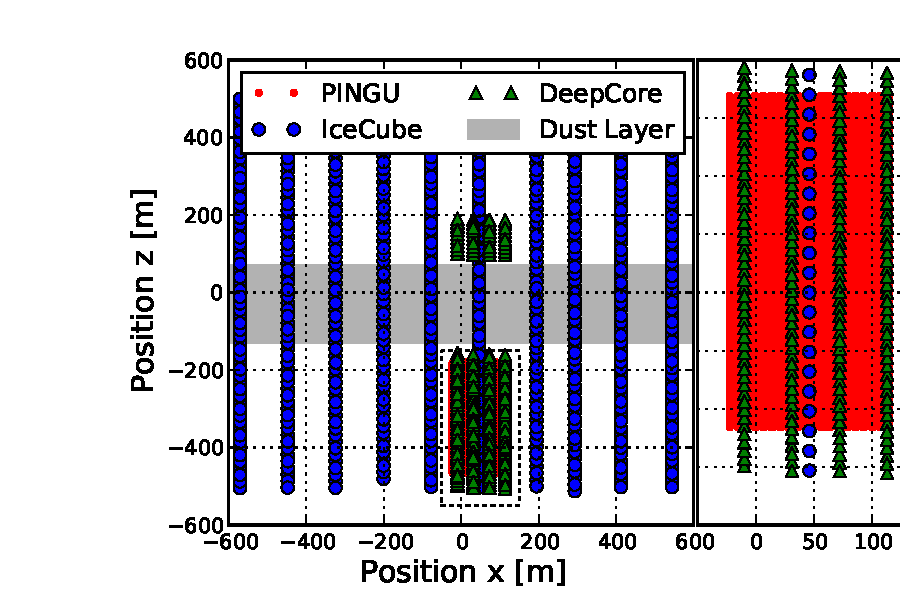
\includegraphics[width=0.8\textwidth]{ic_dc_pingu_sideview}
%  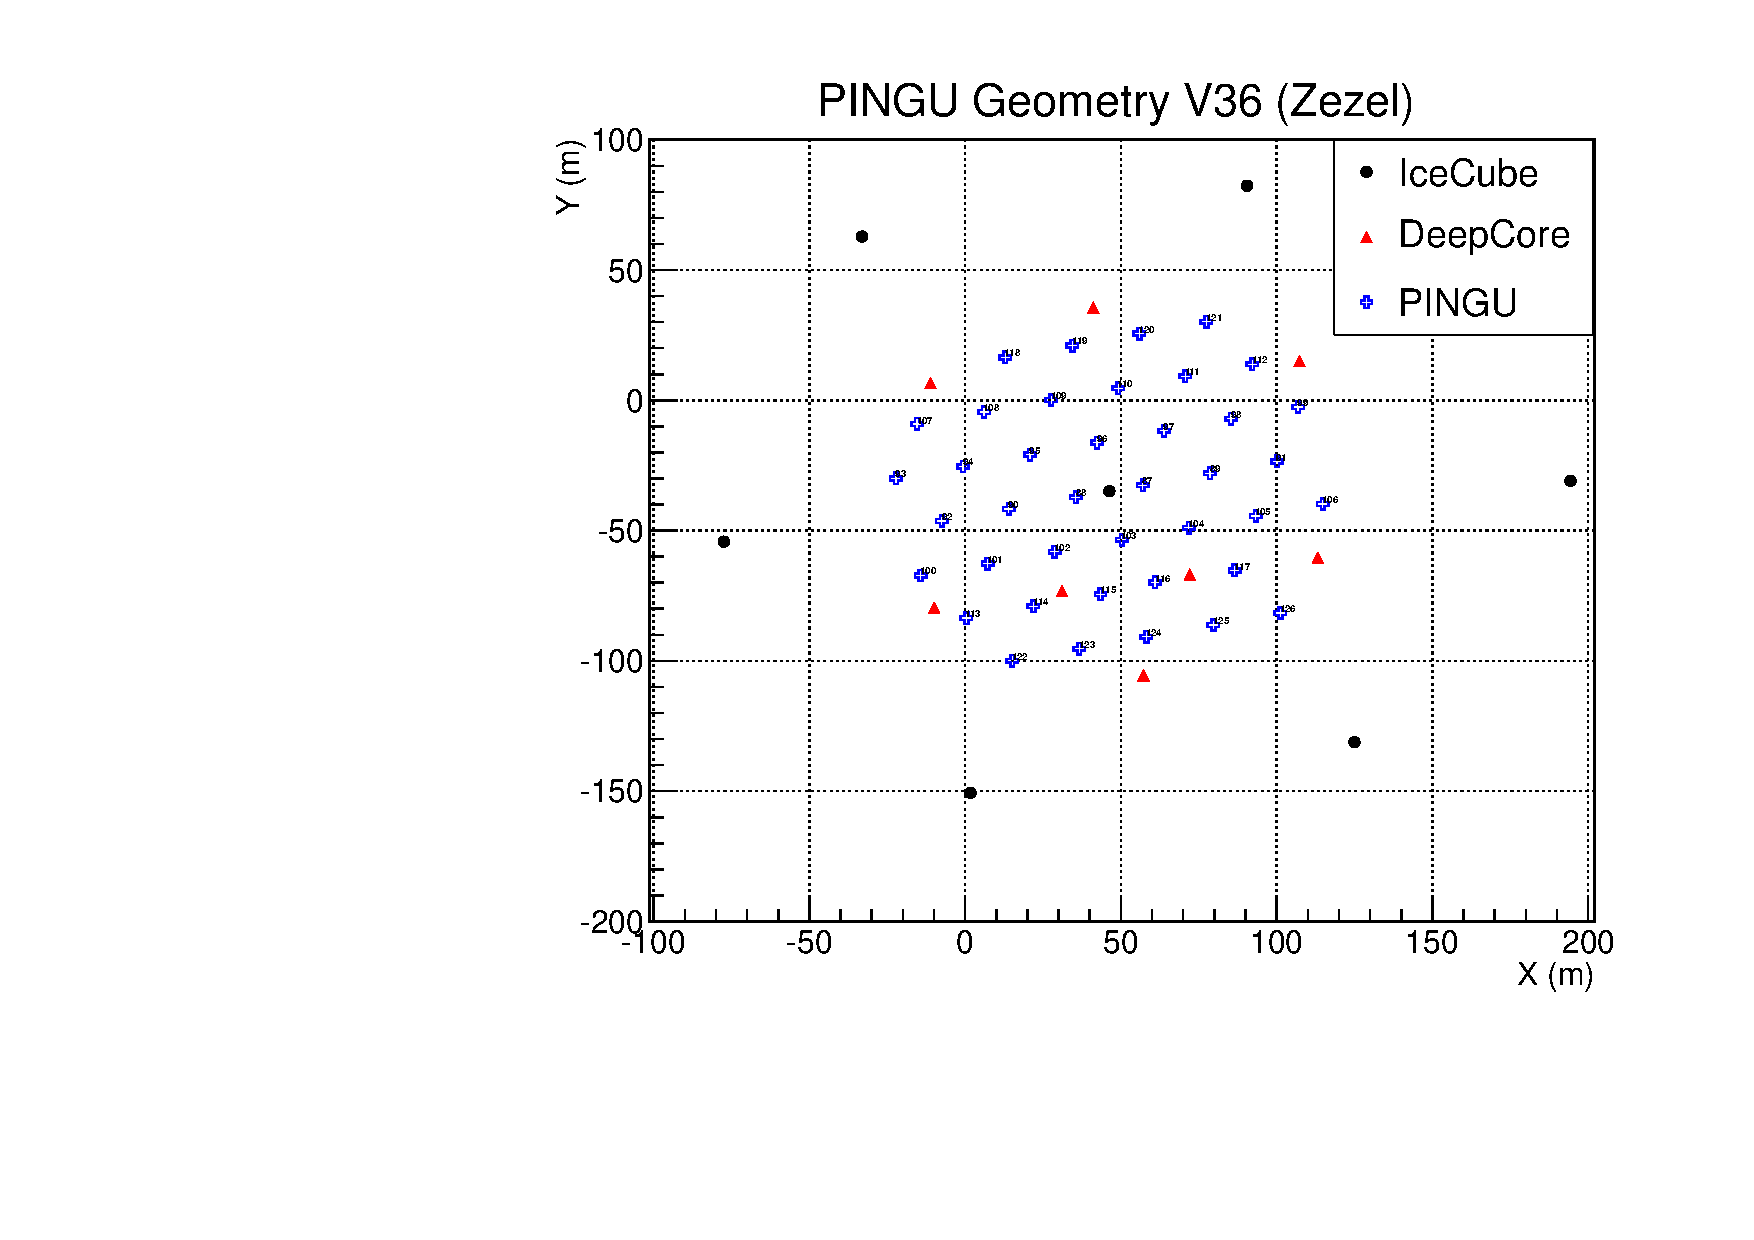
\includegraphics[width=0.7\textwidth]{pingu_V36_Zezel_40_s22_d3}
 \caption{Side view of the IceCube string layout, including the DeepCore and
  planned PINGU (geometry V36) sub-arrays. The approximate position of the dust
  layer is shown for reference.}
 \label{fig:string_layout_side}
\end{figure}

This detector geometry has been optimised to yield a maximum sensitivity for 
the neutrino mass hierarchy. It will be used for all studies described in 
Chapter~\ref{sec:ana} unless explicitly stated otherwise.

In terms of hardware and software infrastructure, many things can be adopted 
from IceCube, redesigning parts where a potential for improvement or 
simplification has been discovered. Several components of the electronics part
of the module, like the main board, the PMT base, and the high voltage supply,
have been redesigned or replaced by more recent versions. In particular the PMTs
will all be the high quantum efficiency models already installed in DeepCore.
A delay board has become obsolete with the more recent signal digitisers and
will not be part of the PINGU DOMs. Additional components, such as cameras to
monitor the freeze-in process, are in discussion.

Although the bulk of PDOMs are an improved version of the technology that has 
proven to work reliably, prototypes of novel optical modules will be deployed 
with PINGU as well. As those might be the baseline technology of future 
neutrino telescopes, they have to be tested under realistic conditions before 
they can be considered for large-scale use. Two options for these 
next-generation optical modules are described in Sec.~\ref{sec:Gen2DOM}, 
studies showing how they will impact the NMH determination are presented in 
Sec.~\ref{sec:om_effects}.

Another thing to be improved upon in PINGU is the so-called ``hole ice''. In 
IceCube it was observed that the refrozen ice directly around the strings that 
had been molten during deployment contains lots of small air bubbles. These 
inclusions lead to a dramatically reduced scattering length around the DOMs,
significantly deteriorating the quality of event reconstruction that strongly
profits from a large number of direct (i.\,e.\ unscattered) photons being
recorded. In order to reduce the impact of the hole ice, the molten water will
be degassed as a part of the drilling process for PINGU, thus reducing its air
content and hence the number of air bubbles remaining after refreezing.

%==============================================================================
\section{Event Reconstruction}
\label{sec:EvtReco}
%==============================================================================

To identify the features in the distribution of neutrino events recorded by
PINGU that are imprinted by the neutrino mass hierarchy, it is crucial to
reconstruct the events as exactly as possible. Although the interesting neutrino
properties are only its energy and the zenith angle of its arrival
direction\footnote{Which determines the length of propagation since the
creation in the Earth's atmosphere and the matter potential passed on the way.}
as those are determining the oscillation probability, an actual neutrino
interaction event in PINGU has far more properties that need to be
reconstructed as well. These are:
\begin{itemize}
 \item The position of the interaction vertex in both space and time, giving
  rise to four variables in total ($x,\,y,\,z,\,t$).
 \item The energy of the hadronic cascade caused by the fragmented target
  nucleus, $E_\mathrm{cscd}$.
 \item The direction of the hadronic cascade, described by its zenith and
  azimuth angles ($\theta,\,\phi$)
 \item The energy $E_\mu$ of the outgoing muon (if present), which can be
  replaced by its length $l$ since muons can be
  considered as minimum ionising particles (see Sec.~\ref{sec:NuDetection}).
 \item The direction of the muon, represented by zenith and azimuth angles
  ($\theta_\mu,\,\phi_\mu$) as well.
\end{itemize}
This amounts to a total of ten variables (seven if no muon is created in the
interaction) whose values have to be found in the reconstruction process. The
neutrino energy is then given by the sum of cascade and muon energy, and its
direction has to be calculated from their momenta using the conservation of the
total momentum. 

\subsection{CLast}
\label{sec:reco_clast}

The start of the reconstruction chain is CLast \cite{CLast}, a first-guess
algorithm for cascade, i.\,e.\ point-like events. With $vec{r}_i$ being the
positions of the DOMs that have registered charges $a_i$ at times $t_i$ in the
event, first the event vertex is determined a the centre of gravity (COG) of the
hit DOMs:
\begin{equation}
 \vec{x} = \sum_i a_i \vec{r}_i
\end{equation}

Following that, the time $t$ of the vertex is calculated. For this, the residual
time is defined as
\begin{equation}
 \tau_i(t) = t_i - \left( t + d_i/c_\mathrm{ice} \right) \quad,
\end{equation}
where $d_i = | \vec{x} - \vec{r}_i |$ and $c_\mathrm{ice} = c/n_\mathrm{ice}$ is
the speed of light in ice. After that, a direct hit is defined as a DOM hit
with $0 < \tau_i < t_w$, with a trigger window of $t_w = 200$\,ns. Now for each
DOM, a test vertex time is chosen to be $t_i - d_i/c_\mathrm{ice}$ and the
number of direct hits on all other DOMs is calculated. From all those test
vertex times, the earliest one resulting in more than four direct hits on other
DOMs is chosen as the vertex time $t$.

After the vertex position has been established, the cascade direction is
determined from the ``tensor of inertia'' of the hit pattern. In a reference
frame centred at the COG, $\vec{r}_i' = \vec{r} - \vec{x}$, this is calculated
analogue to the quantity in classical mechanics with the mass replaced by the
DOM charge:
\begin{equation}
 I^{k,l} = \sum_i a_i \left(\delta^{kl} \vec{r}_i'^2 - r_i'^k r_i'^l\right)
\end{equation}
The cascade direction is then given by the eigenvector corresponding to the
smallest eigenvalue of the tensor of inertia, which points along the strongest
elongation of the hit pattern.

Finally, a first estimate for the cascade energy is calculated using an
empirical polynomial fit \cite{Processing} to the number of hit DOMs in the
event, $N_\mathrm{Ch}$:
\begin{equation}
 \log_{10}\left(E_\mathrm{cscd} [\mathrm{GeV}]\right) =
  -3.3 + x\,(\,9.2 + x\,(\,-9.7 + x\,(\,5.3 + x\,(\,-1.4 + x\cdot 0.134))))
\end{equation}
with $x = \log_{10}(N_\mathrm{Ch})$.

\subsection{Photonics}
\label{sec:reco_photonics}

The Photonics software \cite{Photonics} is a tool widely used in IceCube to get
a fast description of the propagation of Cherenkov photons in the ice. Its main
functionality is to return the expected number of registered photons
$B(\vec{r}, \vec{x}, t, \theta, \phi)$ for any combination of source
$(\vec{x}, t, \theta, \phi)$ and sensor position $\vec{r}$.

Since photon propagation needs extensive computing, $B$ cannot be directly
simulated for each request. The number is retrieved from a table look-up
instead. The respective tables have to be generated in advance by simulating a
large number of sources in all possible depths---since the optical properties
of the Antarctic ice sheet depend strongly on the vertical position, see
Fig.~\ref{fig:ice_scatt_abs}---and all possible zenith angles, using data on the
ice properties that have been retrieved from onboard LED flasher signals
recorded by the IceCube DOMs \cite{Dima}. The resulting photon density
distribution is then stored in six-dimensional tables, the relevant quantities
being three spatial dimensions, the relative time between emission and
detection, the emission angle at the source, and the angle of incidence on the
detector since the DOMs have a zenith dependent detection efficiency, as clearly
visible from their layout (Fig.~\ref{fig:DOM}).

Finally these tables are fitted with multidimensional spline functions, which
leads to more smooth results and significantly reduces the amount of data that
has to be stored \cite{Dima}. This is an important issue, since one of those
six-dimensional tables has to be loaded into the CPU memory for every source
depth, orientation, and type (point-like and track-like, as these have
different light output distributions).

\subsection{Monopod}
\label{sec:reco_monopod}

The Monopod algorithm is an likelihood reconstruction for cascade-like events
using detailed photon timing information. It is the single source case of the
more general Millipede algorithm \cite{Millipede} that is used for high-energy
track reconstruction, where it segments an extended track into a series of
point-like energy depositions along the track.

Assuming a cascade-like energy deposition $E$ at the vertex position $\vec{x}$
and time $t$, pointing into the direction $(\theta, \phi)$, the expected number
of photons $B^\mathrm{cscd}_j(\vec{r}_i, \vec{x}, t, \theta, \phi)$ per unit
energy is retrieved from Photonics (see Sec.~\ref{sec:reco_photonics}) for every
DOM $i$ that registered photons in the event and for every time bin $j$. The
total number of expected photons is then
\begin{equation}
 \mu_{ij} = B^\mathrm{cscd}_j(\vec{r}_i, \vec{x}, t, \theta, \phi)
             \,E_\mathrm{cscd} + \nu_j  \quad, \label{eqn:cscd_hypo}
\end{equation}
where $\nu_j$ is the expectation of noise hits.

From this, a Poisson likelihood is constructed according to
\begin{equation}
 \mathcal{L} = \prod_i^\mathrm{\#\ hit\ DOMs} 
   \quad \prod_{j}^\mathrm{\#\ time\ bins}
   \frac{\mu_{ij}^{n_{ij}}}{\Gamma\left(n_{ij}+1\right)}\ e^{-\mu_{ij}} \quad,
\end{equation}
with $n_{ij}$ being the actual number of photons registered on DOM $i$ in the
time bin $j$. A fitting routine can now search for the values of $(\vec{x}, t,
\theta, \phi)$ that maximise $\mathcal{L}$, corresponding to the most
probable values of the true cascade parameters.

Those fitting routines search for the maximum value of
$\mathcal{L}$\footnote{Usually, and computationally more conveniently, they
search for the minimum of $-\log\mathcal{L}$. Hence they are commonly called
``minimisers''.} in a multidimensional parameter
space in an iterative process. In general, the procedure is to choose a test
point in the parameter space, where the likelihood and its gradient vector are
evaluated. After that, the test point is moved into the direction of the
gradient by a distance depending on its magnitude. This procedure is repeated
until the likelihood difference between two subsequent test points is below a
predefined convergence value, indicating that the minimum has been found, or the
maximum number of iterations has been reached.

In PINGU, Monopod is run with four iterations using the output of CLast as
seed, i.\,e.\ the first test point. Yet obviously it cannot fully describe
all of the expected events since its assumption about the event topology does
not contain the possibility of an outgoing muon track. But since muons at PINGU
energies of few GeV have a range at the order of ten or twenty metres,
comparable to the string spacing, and hence only slightly distort the point-like
event topology. Thus Monopod still gives a reliable estimate of the vertex
position and direction, sufficiently precise for the first loose vertex
containment cut (Sec.~\ref{sec:cuts_step1}). Afterwards it is used as seed for
the more elaborate HybridReco/MultiNest reconstruction.

\subsection{HybridReco/MultiNest}
\label{sec:reco_multinest}

The final, most accurate and involved reconstruction for PINGU events is called
HybridReco/MultiNest, or just MultiNest. It consists of two different
ingredients: the HybridReco event hypothesis and the MultiNest minimiser.

\subsubsection{HybridReco}

To conform to the actual event topology in PINGU, it is necessary to add the
possibility of an outgoing muon of finite length to the pure cascade hypothesis
that was used for the previous reconstructions. Since its starting point is
fixed at the cascade vertex, the muon adds only three variable to the problem:
its direction, again defined by two angles, and its length. However at PINGU
energies the kinematic angle between the hadronic cascade and the outgoing
lepton is only a few degrees \cite{NuScattAng}, far below the directional
resolution of the reconstruction (see Sec.~\ref{sec:sim_input}), the directions
of muon and cascade are assumed to be aligned to reduce complexity. Thus only
the muon energy $E_\mu$, which is proportional to its length, is added to the
set of parameters.

This means that the expression for the expected number of photons on a certain
DOM (\ref{eqn:cscd_hypo}) has to be extended by a term representing the muon
track:
\begin{equation}
  \mu_{ij} = B^\mathrm{cscd}_j(\vec{r}_i, \vec{x}, t, \theta,\phi)
              \,E_\mathrm{cscd}
   + B^\mathrm{track}_j(\vec{r}_i, \vec{x}, t, \theta, \phi)\,E_\mu
   + \nu_j \quad, \label{eqn:hybrid_hypo}
\end{equation}
Although only one variable is added with respect to the cascade reconstruction,
it turns out that finding the maximum likelihood gets much more difficult than
before. The reason for this is the fact that two different photon emission
patterns, $B^\mathrm{cscd}$ for the hadronic cascade and $B^\mathrm{track}$ for
the muon, have to be considered in the hypothesis where it is unclear whether a
given photon originates from the cascade or the muon. Additionally the typical
distances in PINGU are so small that photon scattering plays only a small role
and most of the photons reach the DOMs on an undisturbed path, so-called
``direct hits''.

As an illustration, consider a photon that is detected close to the muon track
in its direction of travel ...

These direct hits cause discontinuities in the likelihood space ...

\subsection{MultiNest}

%==============================================================================
\section{Event Selection}
\label{sec:EvtSel}
%==============================================================================

Since in PINGU the expected rate of neutrino events is in the order of $1 -
2$\,mHz, corresponding to about five neutrinos per hour, while background
events, the vast majority caused by atmospheric muons, will be triggered at
several kHz\footnote{In IceCube, the trigger rate is $\approx 3000$\,Hz.}, an
efficient background rejection algorithm is essential. At the same time, one
has to make sure that a large fraction of the neutrinos carrying the neutrino
mass hierarchy signal pass the imposed cuts---since it is only a second-order
effect event statistics are of great importance---and that the signal in the
data is not destroyed or changed by the cuts.

For the data samples used in this study, a two step selection has been applied
\cite{Processing}. The rationale for this approach is the efficient use of
computing resources. At least the first part of the data reduction has to be run
directly at the South Pole due to the limited bandwidth for data transmission to
the northern hemisphere. Hence the computing for this part has to be
lightweight, as computing resources in Antarctica are scarce as well. After the
easily identifiable background events have been removed, more involved
reconstructions can be run on the remaining data, whose results will be used for
a refined second event selection and eventually in the analysis of the final
data sample.

% \subsection{Trigger and Noise Cleaning}
% \label{sec:cuts_trigger}
% TODO: Write about it?

\subsection{Step 1}
\label{sec:cuts_step1}

The first set of cuts is based on the rather fast CLast and Monopod
reconstructions and on the topology of the charge distribution in the detector
itself. The cut variables have demonstrated their discrimination power in
previous DeepCore analyses, where atmospheric neutrino oscillations have already
been measured at higher energy \cite{DCosc}.

\begin{description}
 \item[$\mathbf{z_\mathrm{CLast} < -200}$\,m:] The very first cut requires the
  event vertex reconstructed by the CLast algorithm to be below --\,200\,m in
  IceCube coordinates, which is 20\,m below the topmost PINGU DOMs. Since
  atmospheric muons enter the detector from above moving downwards, their
  vertices tend to be reconstructed  at the highest possible location while the
  neutrinos that PINGU is interested  in have travelled through the Earth and
  interact inside the detector volume,  pointing upwards.

\item[C2QR6\ $\mathbf{>0.5}$:] The next cut is the so-called ``C2QR6'' quantity
  being  larger than 0.5. It is defined as the fraction of the total PMT charge
  in the  event that has been accumulated within the first 600\,ns, while the
  two very  first hits are ignored. Muons are usually travelling through the
  detector on  an extended path and generate Cherenkov light evenly along it, so
  that usually  only a small fraction of it is recorded during the first
  600\,ns\footnote{During this time, a muon propagates $ct\approx180$\,m.}.
  Neutrinos on the other hand deposit a large fraction of their energy in the
  hadronic cascade that only lasts for few ns.

\item[$\mathbf{z_\mathrm{travel} > -30}$\,m:] For the third cut, the mean spread
  in $z$  of all hits is calculated relative to the mean depth of the first
  quartile of  hits in the event. The cut is passed if this value is larger than
  --\,30\,m,  meaning that the the topology of the event is not too strongly
  pointing  downwards. Again this disfavours muons travelling through the
  detector from  top to bottom while retaining neutrinos coming from below.

\item[$\mathbf{t_\mathrm{90\,\%} < 2}$\,\textmu s:] This cut requires the
  time from  the start of the event after which 90\,\% of the total charge has
  been  accumulated to be less than 2\,\textmu s. Again the reasoning is that
  background muons deposit their energy evenly on their rather long path
  through the  detector, while neutrinos are almost point-like sources in both
  location and  time.

\item[$\mathbf{r_\mathrm{Monopod} < 95}$\,m:] Looking at the secondary 
  Monopod reconstruction, the final cut at the first level secures that the
  event is contained in the detector volume not only vertically, but also
  horizontally. This horizontal containment is considered to be fulfilled if
  the reconstructed vertex is not farther than 95\,m from the detector centre
  at ($50$\,m, $-35$\,m) in the $xy$ direction. The containment assures that
  the event has the possibility to be successfully reconstructed by the
  MultiNest algorithm, which has to be run prior to the second cut level.
\end{description}


\subsection{Step 2}
\label{sec:cuts_step2}

The intention of the second set of cuts is not so much to reject background
events, which is the focus of the first cut level, but rather to select
well-reconstructed events whose quality is sufficient for the final analysis.
Therefore all the cuts in the second step are merely containment cuts, assuming
any non-neutrino event fulfilling the strict containment has already been
recognised and removed in the first step. The reference reconstruction for the
following cuts is the MultiNest reconstruction (Sec.~\ref{sec:reco_multinest})
that has been run on all events passing the first stage of cuts.

\begin{description}
 \item[$\mathbf{-500}$\,m $\mathbf{< z_\mathrm{vertex} < -180}$\,m:] The upper
  bound of the vertical containment, as shown in
  Fig.~\ref{fig:string_layout_side}, has been loosened with respect to the
  $z_\mathrm{vertex} < -200$\,m cut in step one, where the stricter bound was
  necessary due to the strong downgoing background contamination. The lower
  boundary has been introduced since events originating from far below the
  instrumented volume generally have poor reconstruction quality as only
  photons that have travelled far through the ice and hence are subject to
  multiple scattering contribute to the signal recorded in the detector.

 \item[$\mathbf{r_\mathrm{vertex} < 85}$\,m:] The horizontal containment, shown
  in Fig.~\ref{fig:string_layout}, has  been tightened by 10\,m compared to the
  first step. Since the reconstructed  zenith angle of the neutrino is a key
  variable in the mass hierarchy  analysis, one needs to make sure that this
  quantity is reconstructed as accurately as possible. This can not be
  guaranteed for events that are so  close to the edge of the detector that they
  are recorded only partly.

 \item[$\mathbf{\theta_\mathrm{zenith} \geq \pi/2}$ (optional):] For the mass
  hierarchy analysis, neutrinos that have undergone oscillations in a matter
  potential have to be selected. This means that only events that are
  reconstructed as upgoing and hence have passed through the Earth will be
  selected for the final data sample. However, the downgoing neutrino sample
  can still be used as a control region, e.\,g.\ for the normalisation of the
  atmospheric neutrino flux or to estimate the remaining background
  contamination at the final cut level.
\end{description}

\subsection{Particle Flavour Identification}
\label{sec:PID}

%==============================================================================
\section{Next-Generation Optical Modules}
\label{sec:Gen2DOM}
%==============================================================================

Currently two different prototypes of optical modules are supposed to be
deployed in PINGU. The first one, called mDOM (Sec.~\ref{sec:mDOM}), is an
adaptation of the Km3NeT optical module \cite{Km3NeTmodule} whose shape has been
changed from spherical to cylindrical in order to fit into the holes drilled for
the PINGU strings. The other one, called WOM (Sec.~\ref{sec:WOM}), is a novel
approach to enhance the photon collection efficiency by using passive
components.

Both types of modules will be described in more detail below. In
Sec.~\ref{sec:om_effects}, the performance of a PINGU detector consisting fully
of these next-generation modules will be investigated.

\subsection{Multi-PMT Optical Module (mDOM)}
\label{sec:mDOM}

% \begin{figure}[htp]
%  \centering
%  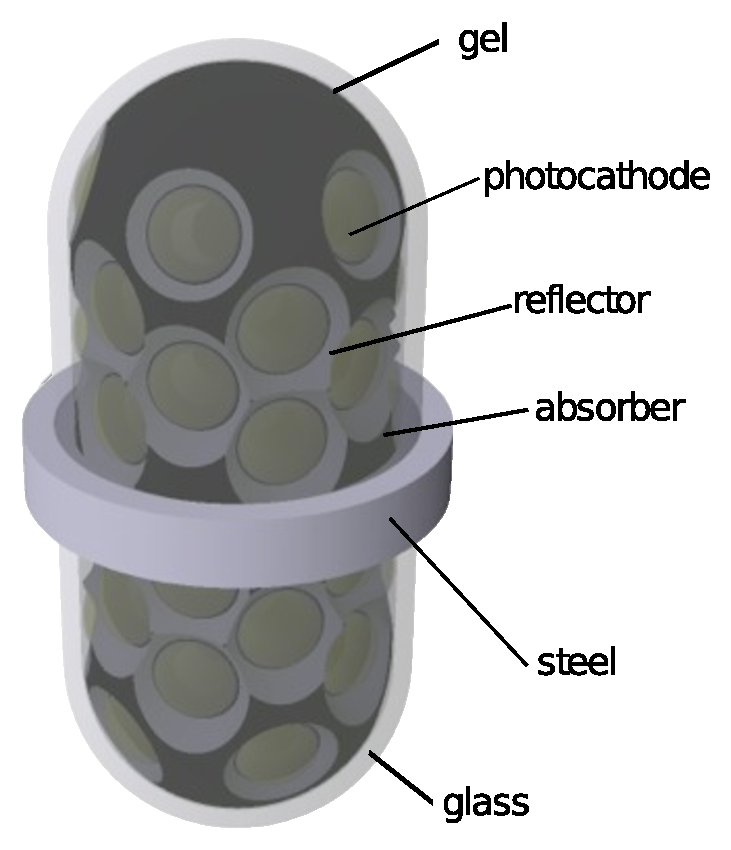
\includegraphics[width=0.5\textwidth]{mDOM_cropped}
%  \caption{The mDOM module concept. Graphics taken from \cite{mDOM_Geneva}.}
%  \label{fig:mDOM}
% \end{figure}

\begin{figure}
\centering
  \subfloat[\label{fig:mDOM}]
    {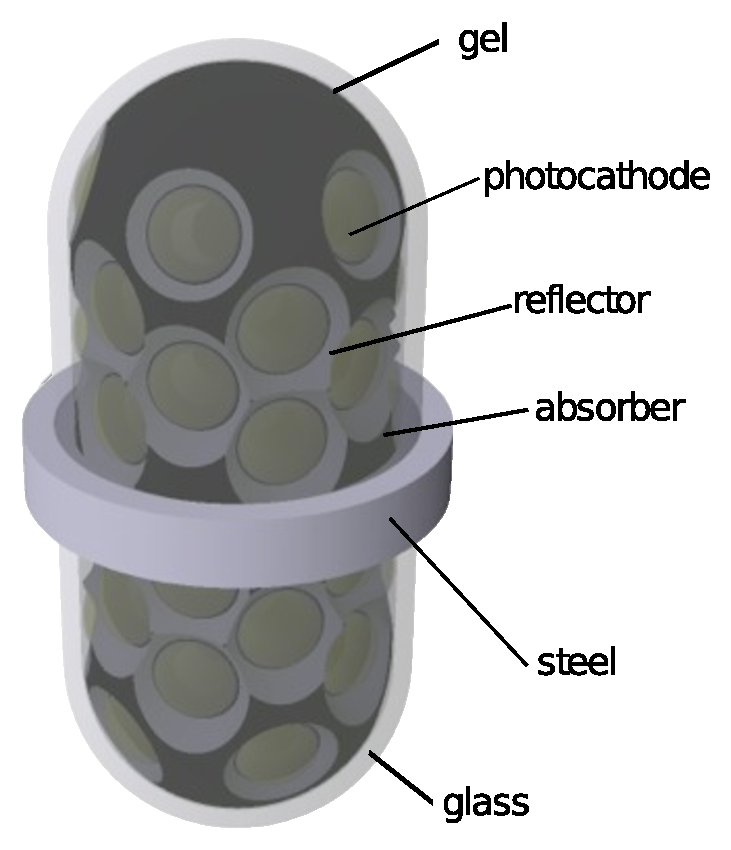
\includegraphics[height=7cm]{mDOM_cropped}}\qquad
  \subfloat[\label{fig:WOM}]
    {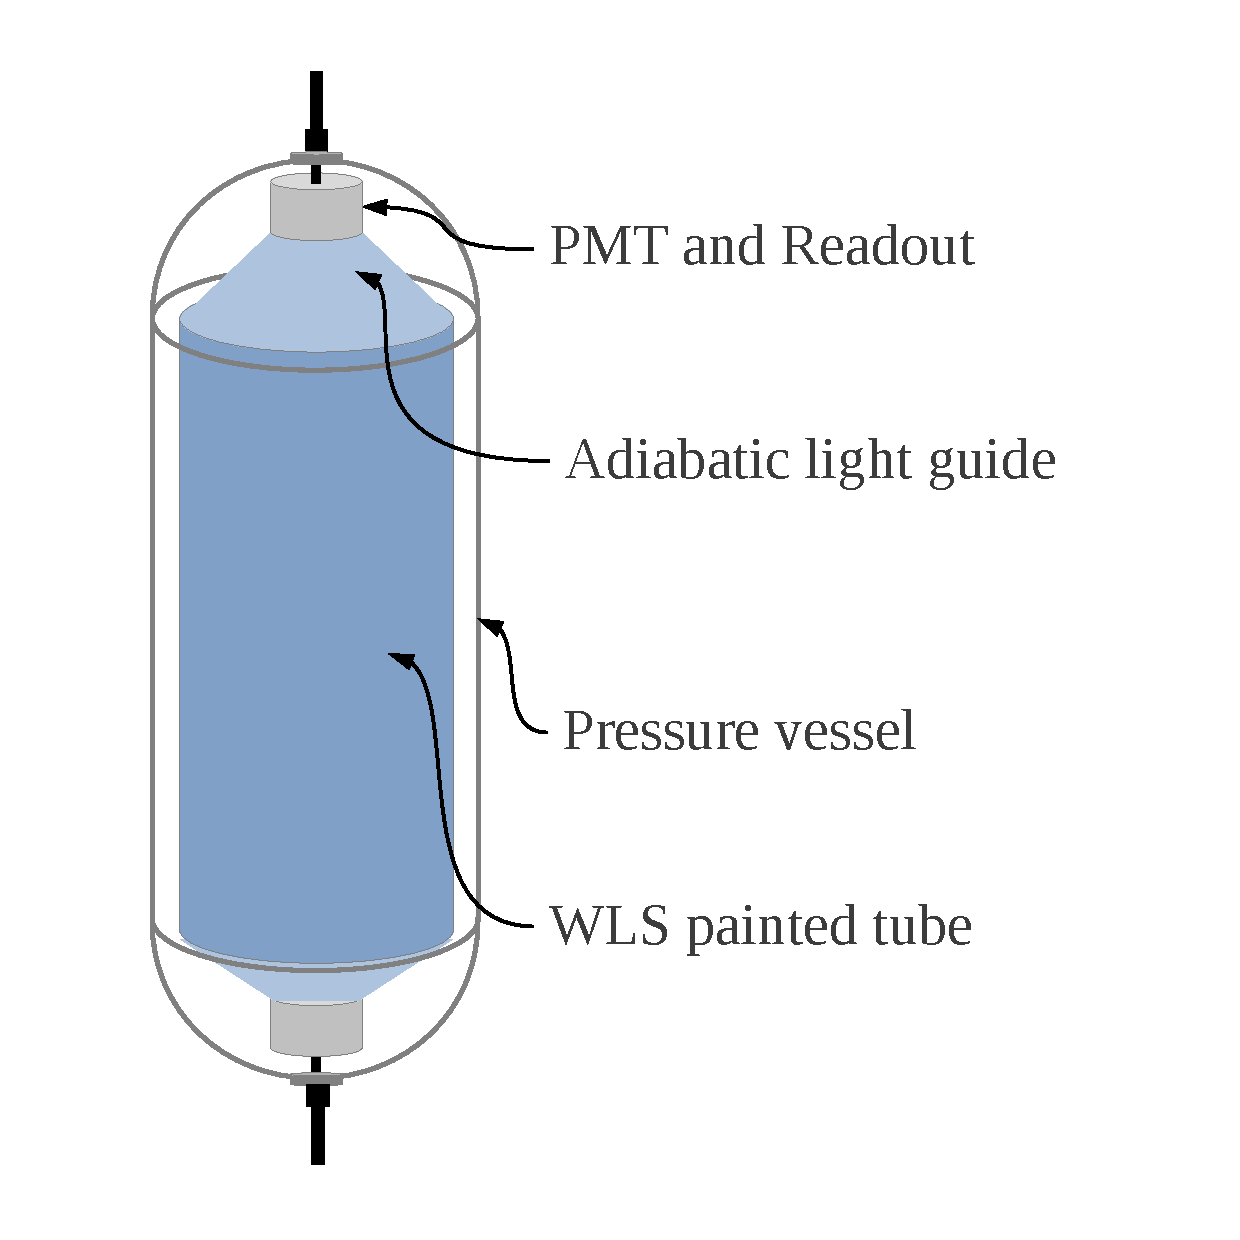
\includegraphics[height=7cm]{WOM}}
  \caption{The \protect\subref{fig:mDOM} mDOM and \protect\subref{fig:WOM} WOM
    module concepts. Graphics taken from \cite{mDOM_Geneva} and \cite{WOM_ICRC},
    respectively.}
\label{fig:Gen3modules}
\end{figure}

Comparing the mDOM, short for Multi-PMT Optical Module, to the standard PINGU
DOMs, the main difference is that instead of one single large PMT, a total of
41 small PMTs with 3\verb+"+ diameter will be used for photon detection, see
Fig.~\ref{fig:mDOM}. The advantages from this layout are that the angular
acceptance covers almost every direction, in contrast to the downwards-pointing
single PMT that has no sensitivity for photons arriving from above
\cite{mDOM_Geneva}.

In addition, the use of more than one PMT per module allows for a very
effective noise reduction. If one only counts module hits where at least two
different PMTs on the same module have registered a photon within a very short
coincidence time, the most important sources of module noise can be strongly
suppressed: Both radioactive decays inside the PMT glass housing and random
electronic noise are restricted to one PMT at a time and hence vetoed with
close to 100\,\% efficiency.

\subsection{Wavelength-shifting Optical Module (WOM)}
\label{sec:WOM}

The WOM on the other hand uses smaller PMTs as well, but enhances the sensitive
area of the module by using passive components as light collectors and
concentrators instead of putting several PMTs into one module \cite{WOM_ICRC}.
The main component, as shown in Fig.~\ref{fig:WOM}, will be a cylindrical tube
made of quartz glass, which has a very low contamination with radioactive
isotopes, that has a coating with wavelength-shifting properties.

In this coating, Cherenkov photons, which are mostly in the UV range (cf.\
Sec.~\ref{sec:Cherenkov}), will be absorbed and then re-emitted isotropically
at a larger wavelength. Due to this isotropic emission a large fraction of the
photons, which were incident roughly perpendicular to the cylinder surface,
will be captured within the tube and hence guided towards its end via multiple
total internal reflection. At the end of the tube, an adiabatic light guide
will project its cross-section area onto a small PMT which then reads out the
photons. Since their spectrum has been shifted from the UV to the optical blue,
it is now better suited for readout by conventional PMTs which are usually most
sensitive for the blue and green part of the optical regime.

In this setup, the size of the sensitive area is given by the coated quartz
glass tube, whose dimensions, especially the length, can be scaled up almost
arbitrarily. At the same time the module noise is dominated by the single PMT
at $\mathcal{O}$(10\,Hz) \cite{WOM_ICRC}, since the quartz glass housing and the
organic wavelength shifter are passive components without electronic noise, and
their radioactive contamination is negligible. So in contrast to the mDOM, the
WOM can fully exploit its large sensitive area to increase the photon
statistics, while in the former the larger sensitive area gets eaten up by the
fact that only multiple photon hits on the same module are counted.